\chapter{聚类与 k-means 算法}

在聚类问题中,给定一个训练集 $\{x^{(1)}, \dots, x^{(n)}\}$,我们希望将数据分组到一些具有汇聚效果的“簇”中。这里,$x^{(i)} \in \mathbb{R}^d$ 像往常一样,但没有给出标签 $y^{(i)}$。因此,这是一个无监督学习问题。

$k$-means 聚类算法如下:

\begin{enumerate}
    \item 随机初始化\textbf{簇中心 (cluster centroids)} $\mu_1, \mu_2, \dots, \mu_k \in \mathbb{R}^d$。
    \item 重复直到收敛:\{
        \begin{itemize}
            \item[] 对于每个 $i$,设置
            \[
                c^{(i)} := \arg \min_j \|x^{(i)} - \mu_j\|^2.
            \]
            \item[] 对于每个 $j$,设置
            \[
                \mu_j := \frac{\sum_{i=1}^n {1}\{c^{(i)} = j\} x^{(i)}}{\sum_{i=1}^n {1}\{c^{(i)} = j\}}.
            \]
        \end{itemize}

    \}
\end{enumerate}

在上述算法中,$k$(算法的一个参数)是我们想要找到的簇的数量;而簇中心 $\mu_j$ 代表我们对簇中心位置的当前猜测。为了初始化簇中心(在上述算法的步骤 1 中),我们可以随机选择 $k$ 个训练样本,并将簇中心设置为这些 $k$ 个样本的值。(也可以采用其他初始化方法。)

算法的内循环重复执行两个步骤:(i) 将每个训练样本 $x^{(i)}$ “分配”给最近的簇中心 $\mu_j$;(ii) 将每个簇中心 $\mu_j$ 移动到分配给它的点的均值。图 \ref{fig:10.1} 展示了 $k$-means 算法运行的示意图。

\begin{figure}[H]
    \centering
    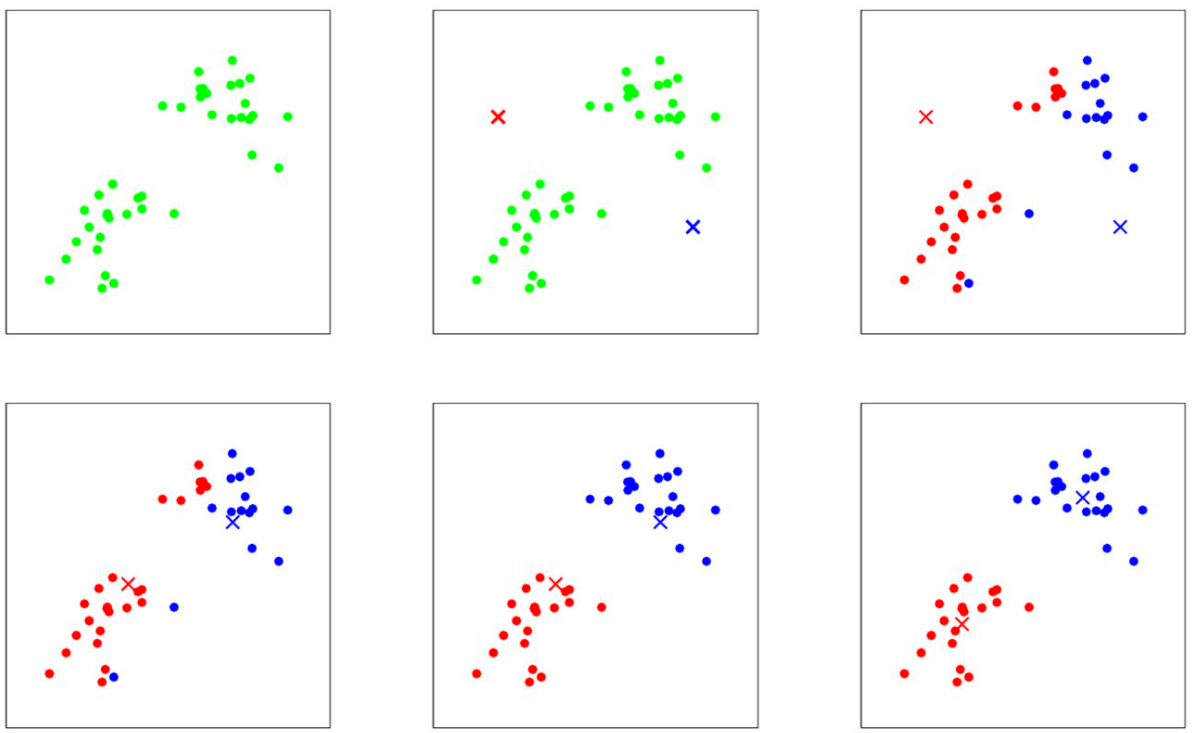
\includegraphics[width=0.9\textwidth]{figs/k-means.png}
    \caption{K-means 算法。训练样本显示为点,簇中心显示为叉。(a) 原始数据集。(b) 随机初始簇中心(在此示例中,不是选择了两个训练样本作为簇中心)。(c-f) 演示运行两次 $k$-means 迭代。每次迭代将每个训练样本分配给最近的簇中心(通过将训练样本“涂成”与其分配到的簇中心相同的颜色来显示);然后我们将每个簇中心移动到分配给它的点的均值。(彩色观看效果最佳。)图片由 Michael Jordan 提供。}
    \label{fig:10.1}
\end{figure}

$k$-means 算法是否保证收敛?是的,在某种意义上。特别地,定义\textbf{失真函数 (distortion function)} 为:
\[
    J(c, \mu) = \sum_{i=1}^n \|x^{(i)} - \mu_{c^{(i)}} \|^2
\]
因此,$J$ 度量了每个训练样本 $x^{(i)}$ 与其被分配到的簇中心 $\mu_{c^{(i)}}$ 之间的平方距离之和。可以证明,$k$-means 正是 $J$ 上的坐标下降。具体来说,$k$-means 的内循环在固定 $\mu$ 的同时重复最小化 $J$ 关于 $c$,然后在固定 $c$ 的同时最小化 $J$ 关于 $\mu$。因此,$J$ 必须单调递减,并且 $J$ 的值必须收敛。(通常,这意味着 $c$ 和 $\mu$ 也会收敛。理论上,$k$-means 算法可能会在几个具有完全相同的 $J$ 值的不同聚类之间振荡,即 $c$ 和/或 $\mu$ 具有几个不同的值,但这在实践中几乎从未发生过。)
失真函数 $J$ 是非凸的,因此在 $J$ 上的坐标下降不保证收敛到全局最小值。换句话说,$k$-means 容易受到局部最优的影响。尽管如此,$k$-means 通常工作良好并能得到很好的聚类结果。但是,如果担心陷入糟糕的局部极小值,常见的做法是多次运行 $k$-means(使用不同的随机初始簇中心 $\mu_j$)。然后,在所有找到的不同聚类中,选择失真 $J(c, \mu)$ 最低的那一个。